\documentclass[a4paper, 12pt]{article}

\usepackage[portuges]{babel}
\usepackage[utf8]{inputenc}
\usepackage{amsmath}
\usepackage{indentfirst}
\usepackage{graphicx}
\usepackage{multicol,lipsum}
\usepackage{hyperref}
\hypersetup{
    colorlinks=true,
    linkcolor=blue,
    filecolor=magenta,      
    urlcolor=cyan,
}

\begin{document}
%\maketitle


	\begin{center}
	
		\vspace{15pt}
        \vspace{95pt}
        \textbf{\LARGE{Análise de Componentes Independentes}}\\
	
		\vspace{3,5cm}
	\end{center}
	
	\begin{flushleft}
		\begin{tabbing}
			Aluno: Samuel Cavalcanti \\
	\end{tabbing}
 \end{flushleft}

%%%%%%%%%%%%%%%%%%%%%%%%%%%%%%%%%%%%%%%%%%%%%%%%%%%%%%%%%%%

% % % % % % % % %FOLHA DE ROSTO % % % % % % % % % %

% % % % % % % % % % % % % % % % % % % % % % % % % %


% % % % % % % % % % % % % % % % % % % % % % % % % % %
\section{Breve descrição do algortimo}  
O algoritmo FastICA pode ser derivado tanto para o caso de maximizar a não-
gaussianidade utilizando o método kurtosis quanto o método negentropia. A diferença
básica entre os algoritmos será a iteração que calculará o novo w. Abaixo segue o algoritmo
utilizando o método negentropia\\
\textbf{1}. Escolher um vetor de pesos w inicial (por exemplo, aleatoriamente). \\
\textbf{2}. $ W^* \longleftarrow  E\{zg(w^tz)\} - E\{zg^{'}(w^tz)\}w $ \\
\textbf{3}. $w \longleftarrow \frac{w^*}{ \Arrowvert  w^*  \Arrowvert }$ \\
\textbf{4}. Se não convergiu, voltar ao passo 2.\\

Como função $g$ as derivadas das funções descritas nas equações \ref{eq1} e \ref{eq2}
podem ser utilizadas (equações \ref{eq3} e \ref{eq4}), pois resultam em boas aproximações da
negentropia. Além dessas funções, pode-se utilizar também a derivada do momento de
quarta ordem, que resultará no método kurtosis (equação \ref{kurtis}).

\begin{equation}\label{eq1}
G_1(y) = \frac{1}{a_1}log(cosh(a_1y))
\end{equation}

\begin{equation}\label{eq2}
G_2(y) = -e^{-\frac{y^2}{2} }
\end{equation}

\begin{equation}\label{eq3}
g_1(y) = tanh(a_1y)
\end{equation}

\begin{equation}\label{eq4}
g_2(y)= \frac{y}{2}e^{-\frac{y^2}{2}}
\end{equation}

\begin{equation}\label{kurtis}
g_3(y) = y^3
\end{equation}


O critério de convergência é o novo e antigo w apontarem para a mesma direção
(considerando que $w$ e $-w$ são iguais.\\
Abaixo seguem algumas propriedades do algoritmo FastICA:\\

\textbf{1.} A convergência é cubica (ou pelo menos quadrática), sob a suposição do modelo de
dados ICA. Isto contrasta com outros algoritmos ICA baseados em métodos de
gradiente descendente, onde a convergência é somente linear. Isto significa uma
rápida convergência para o algoritmo FastICA. Diversos experimentos em dados em
tempo real comprovam esta propriedade.\\

\textbf{2.} Contrário a algoritmos baseados em gradiente, não há nenhum parâmetro de taxa de
aprendizagem para escolher, o que torna o FastICA mais simples.\\

\textbf{3.}O algoritmo encontra diretamente as componentes independentes de praticamente
qualquer distribuição não-gaussiana usando qualquer medida de não-linearidade g,
ao contrário de muitos algoritmos onde a medida de não-linearidade precisa ser
escolhida especificamente\\

\textbf{4.} O desempenho do algoritmo pode ser melhorado com a escolha adequada de uma
medida de não-linearidade.\\

\textbf{5.}As componentes independentes podem ser estimadas uma a uma, o que diminui o
custo computacional em casos onde somente algumas das componentes independen-
tes precisam ser estimadas.\\

\textbf{6.}O algoritmo FastICA possui outras vantagens como: paralelismo, é distribuido, com-
putacionalmente simples e requer pouco espaço de memória. \\

\cite{lamport94}
\section{Problema Exemplo}
O trabalho escolhido foi sobre o ICA. Mais precisamente sobre o fastICA.  
Nesse exemplo o \href{https://scikit-learn.org/stable/auto_examples/decomposition/plot_ica_blind_source_separation.html#sphx-glr-auto-examples-decomposition-plot-ica-blind-source-separation-py}{scikit-learn}
mostra o funcionamento do Fast ICA em comparação com o PCA para a separação de 3 sinais combinados. Nesse exemplo podemos observar que PCA não consegue separar as 3 fontes por causa da não-gaussianidade da amostra. No Entanto o Fast ICA conseguiu.  

\begin{figure}
\caption{scikit-learn exemplo}
\hspace*{-5.5cm}
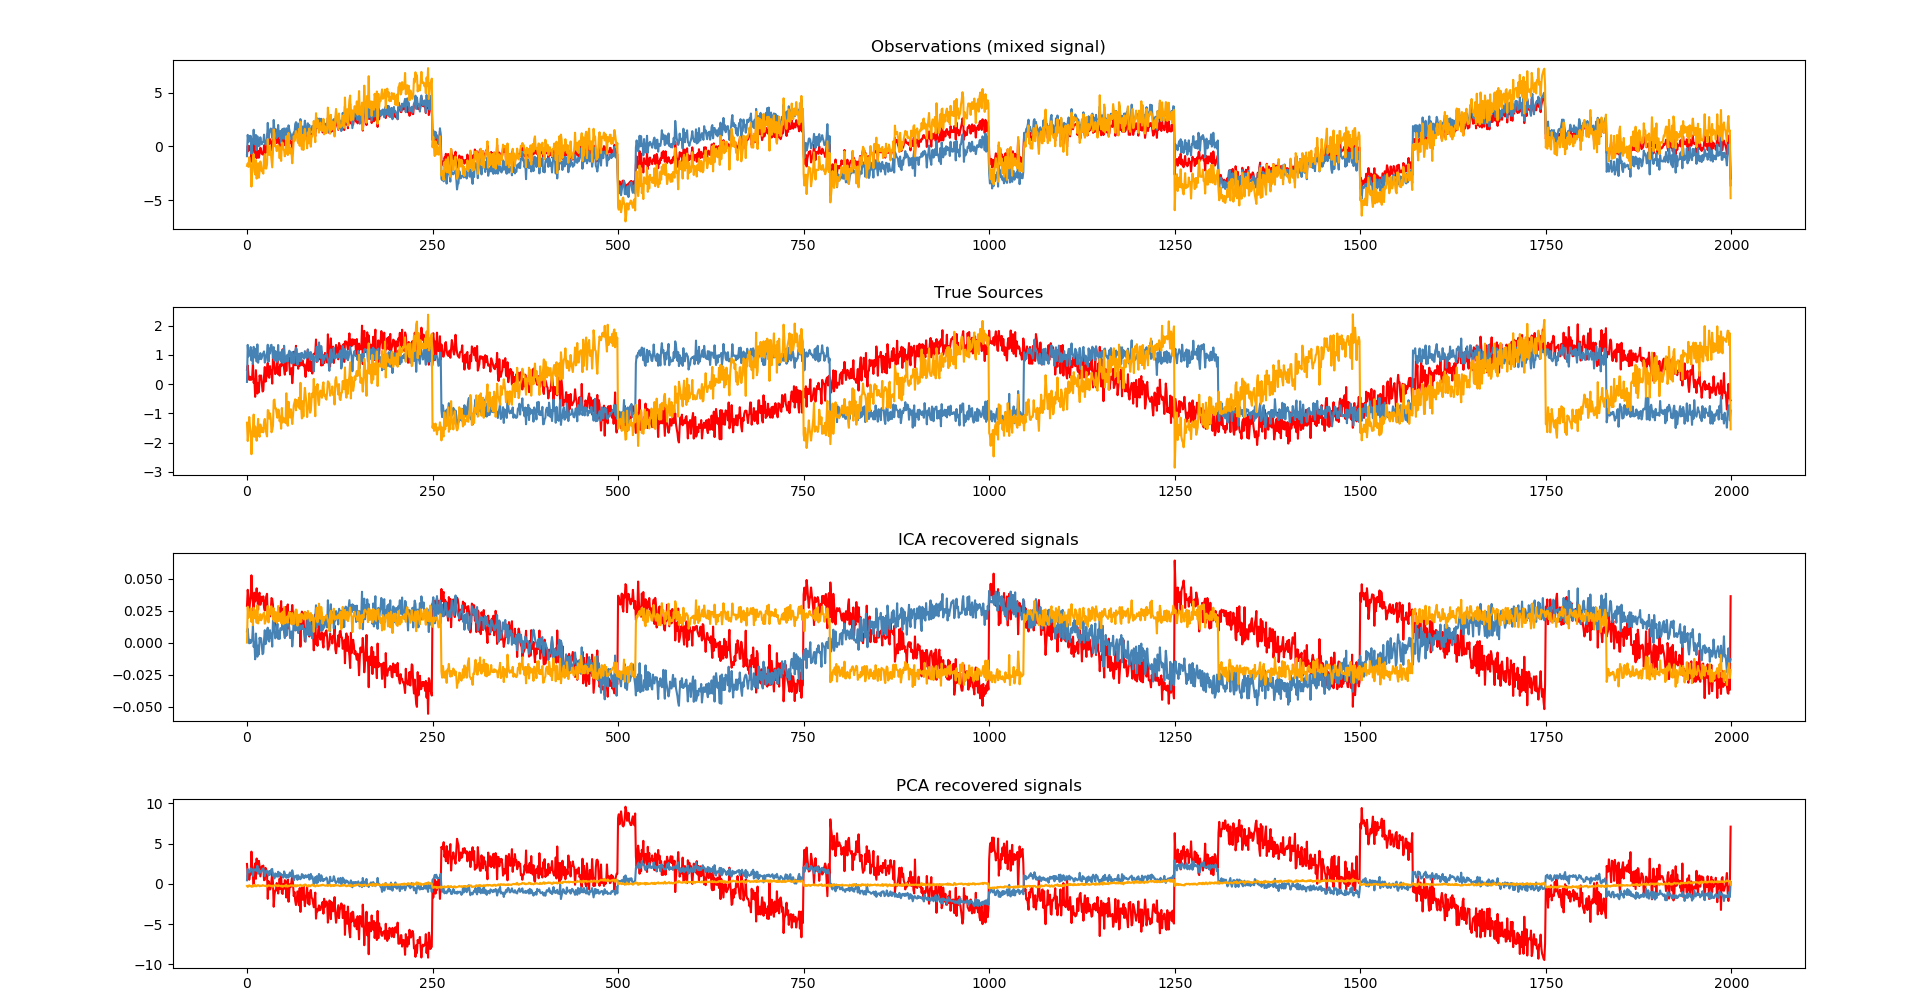
\includegraphics[width=1.8\textwidth]{images/ica_exemple.png}
\end{figure}

\begin{thebibliography}{9}
\bibitem{lamport94}
  Silva, Alan Paulo Oliveira,
  \textit{Uma implementação da análise de componentes independentes em plataforma de hardware reconfigurável},
   Universidade Federal do Rio Grande do Norte,
  2010.
\end{thebibliography}

\end{document}

